\documentclass[letterpaper,10pt,draftclsnofoot,onecolumn]{IEEEtran}
\usepackage{graphicx}
\usepackage{amssymb}
\usepackage{amsmath}
\usepackage{array}
\usepackage{amsthm}
\usepackage{listings}
\usepackage{alltt}
\usepackage{float}
\usepackage{color}
\usepackage{url}
\usepackage{setspace}
\usepackage{balance}
\usepackage{enumitem}
\usepackage{pstricks, pst-node}
\usepackage{inputenc}
\usepackage[margin=.75in]{geometry}

\lstset
{ %Formatting for code in appendix
    %frame=single,
    basicstyle=\footnotesize\ttfamily,
    numbers=left,
    numbersep=.25in,
    stepnumber=1,
    showstringspaces=false,
    tabsize=4,
    breakatwhitespace=false,
    xleftmargin=.5in,
    xrightmargin=.5in,
}

% JS options pulled from https://tex.stackexchange.com/questions/89574/language-option-supported-in-listings
\lstdefinelanguage{JavaScript}{
  keywords={typeof, new, true, false, catch, function, return, null, catch, switch, var, if, in, while, do, else, case, break},
  keywordstyle=\color{blue}\bfseries,
  ndkeywords={class, export, boolean, throw, implements, import, this},
  ndkeywordstyle=\color{darkgray}\bfseries,
  identifierstyle=\color{black},
  sensitive=false,
  comment=[l]{//},
  morecomment=[s]{/*}{*/},
  commentstyle=\color{purple}\ttfamily,
  stringstyle=\color{red}\ttfamily,
  morestring=[b]',
  morestring=[b]"
}

%crappy error with titlesec
\newcommand{\subparagraph}{}
\usepackage{titlesec}

\usepackage{fancyhdr}
\usepackage{hyperref}
\usepackage{tocloft}

%hide toc subsubsections
\setcounter{tocdepth}{2}
\setlength{\parindent}{.25in}

%toc formatting standards
\renewcommand{\cftsecleader}{\cftdotfill{\cftdotsep}{\vspace{.25cm}}}
\renewcommand{\cftsecfont}{\normalfont}
\renewcommand{\cftsecpagefont}{\normalfont}
\renewcommand{\cftsecaftersnum}{.}

%bottom right page numbers
\fancyhf{}
\renewcommand{\headrulewidth}{0pt}
\rfoot{\thepage}
\pagestyle{fancy}

%formatting Section headings
\titleformat{\section}[block]
  {\fontsize{12}{12}\bfseries\sffamily}
  {\thesection.}
  {1em}
  {\vspace{.1cm}}
\titleformat{\subsection}[block]
  {\fontsize{12}{15}\slshape\sffamily}
  {\thesubsection}
  {1em}
  {\vspace{.1cm}}
\titleformat{\subsubsection}[block]
  {\fontsize{11}{20}\slshape\sffamily}
  {\thesubsubsection}
  {1em}
  {\vspace{.1cm}}
  
\geometry{textheight=8.5in, textwidth=6in}

\renewcommand{\thesection}{\arabic{section}}
\renewcommand{\thesubsection}{\thesection.\arabic{subsection}}
\renewcommand{\thesubsubsection}{\thesubsection.\arabic{subsubsection}}

\newcommand{\cred}[1]{{\color{red}#1}}
\newcommand{\cblue}[1]{{\color{blue}#1}}

\def\name{Charles Siebert}

%% The following metadata will show up in the PDF properties
\hypersetup{
  urlcolor = black,
  pdfauthor = {\name},
  pdfkeywords = {cs463 ``Senior Capstone - Spring 2017'' capstone},
  pdftitle = {CS 463 Progress Report - Spring 2017},
  pdfsubject = {Capstone Progress Report - Spring 2017},
  pdfpagemode = UseNone
}

\begin{document}
\begin{titlepage}
\centering
\vspace*{4cm}
{\scshape\LARGE \begin{singlespace}Optimizing Virtual Reality and Augmented Reality Performance on Mobile Web Applications \\ \end{singlespace} \smallskip Group 52 - Progress Report } \\
	{\scshape\Large CS463 - Spring 2017 \par}
	\vspace{.5cm}
	\name \par
    {\large May 15, 2017 \par} 
	\vspace*{1cm}
	
\begin{abstract}
The technology to experience the new trend of Virtual Reality (VR) is not cost effective in today's market. To experience VR, one must pay for the headset and the hardware to run it; this setup can have a combined total of over \$1000, making it inaccessible to a majority of the world's population. Additionally, developers are focusing primarily on expensive high-end high-performance hardware over mobile development for the Augmented Reality (AR) and Virtual Reality (VR) experiences. However, smart phones are currently among some of the mostly widely owned products in the world, meaning there is a much larger potential market for mobile development. Developing AR/VR for the mobile-web platform allows more developers to enter the field to create a better and more stable experience, which then will allow VR to be more accessible to the world. To accomplish this, we are working on a project called �Mobile AR/VR Performance�, which focuses on researching to profile and identify performance bottlenecks in a current 3D web-development framework on mobile devices. We will log and post issues found in mobile browsers such as Chrome and Firefox throughout our time working with A-Frame and Three.js. These issues will pinpoint where there are current bottlenecks in regards to applicable scenarios one might find in an actual VR environment. We hope that our findings will be able to aid in the understanding of the constraints in current mobile technologies when it comes to VR and AR and we hope that future VR teams will be able to learn from our findings to better improve the mobile experience. 
\end{abstract}

\end{titlepage}

\newpage

\thispagestyle{empty}
\pagenumbering{gobble}

\tableofcontents

\cleardoublepage
\pagenumbering{arabic}

\newpage

\begin{singlespace}

\section{Purpose and Goals}
This paper is a progress report for group 52, "OVRAR" over the past 6 weeks for the Spring Term for 2017. Our group has finished the development for our project and has pushed out our final results to our client in the form a blog post to their industry research site.

The purpose of this project is to determine areas of development within A-Frame where there are certain hardware bottlenecks when it comes to applicable mobile development cases, as what we find will need to resemble what the framework will actually be used for. This project is focused towards the advancement of an open-source, mobile web framework, and the developers making their own products with A-Frame in regards to mobile devices. The developers will be using our project research as a means to avoid these bottlenecks in this evolving environment in addition to understand how they can be improved. Developers other than us will use the information in the final report to determine the best way to approach designing their own mobile-web programs, as the software we create will only serve as to stress test and pinpoint current roadblocks.

Our team, Optimizing VR and AR for Mobile Web Apps, was set out to determine Virtual Reality (VR) and Augmented Reality (AR) bottlenecks that exist in mobile devices within the A-Frame framework. The bottlenecks can be caused from either unoptimized development of software, underpowered or unoptimized hardware found in existing devices, or potential bugs or limitations found within the framework itself. The software itself, which is developed on A-Frame, will generate multiple scenes where it will test the graphical capabilities of the hardware within the mobile devices, the types of different implementations of certain scenes, and determine areas of optimization through these multiple scenes. The software will be used to create a report that will analyze the information collected about processing power, frame rates, battery usage, and the limitations of the framework to determine the best practices for implementing more graphically intensive programs on A-Frame.

\section{Group Reports}
Over the past 6 weeks, each of us has submitted weekly updates to describe the progress over the past week, the problems we encountered during the week, and the plans we have for the next week. This is to keep track of our progress as we move through the project time-line, and determine whether we are on track, or behind our current schedule.

\subsection{Charles Siebert}
The following sections include weekly summaries and a retrospective reflection over the past 6 weeks for Charles Siebert.

\subsubsection{Weekly Summaries}
For the first week back, we talked with our client about our current progress, and where we're at with development and how we will proceed with testing. Gave us good feedback based on how we've been moving forward with development, and sounded pretty optimisitic. Over the next week, we will be working with our client to approve the poster we have worked on. There is a second draft of it due soon, and we will need to discuss with our client over any potential brandings they may need to have presented as well. The problems we may run into is getting our test data lined up and ready to determine what we need to find to write and publish our results.

In the second week, we worked on ironing out some finals bugs before testing. I worked on finding a proper model to compare against our original, and finding out how many trees I would need to put into the scene when comparing the vertices of each model that needs to be drawn. We are close to finishing the final development so we can test and compare all of our scenes together. Over the next week we plan to get together and discuss the test cases we have, and how we will draw conclusions for the results we see. We need to talk to our client about our draft of our poster, as it will have industry represented logos on the poster, and determine if it is appropriate to display at the convention. However, we are finishing up our last weeks in this project.

Starting in the third week, we are talking with our client about getting our poster approved, and determining whether or not Mozilla needs any specific branding associated with our poster. As we work on final revisions of this, we are planning out doing some extra credit down the line to do with another group, to practice presenting our projects. We're finishing up the last of our rooms to push towards testing.

During the fourth week, we were given the assignment to do a WIRED style article with another group member. Having to interview another classmate in a different group and write about it will help prepare for a different style of writing. As I'm not used to an article style of writing, it is good practice for when we have to write our blog post for Mozilla, as that is one of our main deliverable products for our client. Though having to do it during the code freeze makes it difficult to prioritize everything properly. Over the next week, we have to finish our code before the code freeze hits, and make sure everything is submitted. That means we have to have our poster ready, approved, and submitted. The troubles we may find over the next week is getting everything submitted and finished on time, as we also have to plan our interviews with other classmates.

This week, we worked on finishing the code on our project for Monday, as that was the code freeze. The previous week, we were given group member's to do the WIRED article, which required us to interview other people and talk about our projects. Earlier in the week, we also met with our client to discuss the project, and our poster. He also discussed the plans of doing a Mozilla blog post to wrap up the project, which will discuss an abstracted overview of our entire project and our results. We are currently working on fine turning our results data in the next week, and prepare this information for expo and our article for our client. The problems we will face into is getting all of the writing done, as we will have another set of progress reports that we will have to write out, on top of preparing for expo and delivering the rest of our requirements to our client.

This week, I worked on getting a Blog article written up to our client to submit for our project. It depicted our approach and resolution based on our testing that we did. Currently working on setting up an account for the Hacks Blog website and submit it for revisions before we can post it. For the next week, we have to get our midterm progress report completely up to date. Have to gather up recording and render a quick video to go with the writing. After that, we have to confirm that we are getting all of the materials we need to prepare for EXPO, which is coming this Friday. Maybe a little practice on our pitches might benefit us... The troubles I see facing the next week is getting this midterm progress report finished, as we have to record and render a new video, on top of submitting a document. Also EXPO is leaving me a little nervous, as it's finally happening.

\subsection{Branden Berlin}
The following sections include weekly summaries and a retrospective reflection over the past 6 weeks for Branden Berlin.
	
\subsubsection{Weekly Summaries}
The first week was spent meeting with our client to catch up from Spring break with any edits or changes we have made, as well as discussing our idea for gathering data. We went over our current design of testing certain features in each room, and how we are going to be doing that. We mentioned we are going to be utilizing Mozilla Beta's dev tools to record the data in our virtual scenes and have them output to a JSON file. Additionally, we will then convert the data to excel and create comparisons. This idea went over well so far, but I think we will truly understand what we are doing only when we begin, because we aren't entirely positive what it is we will encounter until we start our testing. So this next week will be spent planning our test dates and our meet-ups.

This next week was spent meeting with our client to catch up from Spring break with any edits or changes we have made, as well as discussing our idea for gathering data. We went over our current design of testing certain features in each room, and how we are going to be doing that. We mentioned we are going to be utilizing Mozilla Beta's dev tools to "record" the data in our virtual scenes and have them output to JSONS. Additionally, we will then convert the data to excel and create comparisons. This idea went over well so far, but I think we will truly understand what we are doing only when we begin, because we aren't entirely positive what it is we will encounter until we start our testing. So this next week will be spent planning our test dates and our meet-ups.

For the third week, we planned to create some additional rooms to aid in our testing. We realized that our current rooms don't actually cater to real VR scenarios. The purpose of VR is to create a virtual world and our rooms don't exactly resemble something that would be used. So we are planning to begin a second iteration of the rooms that use each feature the room is testing, but in a more realistic scenario. This way, we can add some context to the issues we find. Additionally, we were not able to meet with our client but had a steady email stream and he approves of everything thus far. For the next week we hope to have these new rooms finished for testing.  

During this fourth week we spent finishing most of our development before the freeze. We needed to add a few extra rooms to allow us to do additional testing against the purpose of each room, without changing the fundamentals of the originals. Additionally we began some of our testing and gathering of data. We were not able to meet with our client however he was able to send us the approved logo needed for our poster. We hope to finish our coding by Sunday and then finish up our testing mid-next week so we can begin reading the pulled data. Additionally we will submit our final poster for printing and meet together to discuss the next assignment. Personally, I worked on the second iteration for Room 3 (which was my original). What I did was turn each sphere into a light source with maximum intensity. To turn it one, the user would look at the sphere which would then illuminate the room. With multiple spheres, we will be able to understand at which point the room will malfunction when dealing with multiple light sources. 

The fifth was spent mostly just working on data gathering and the WIRED article. We turned in an approved version of our final poster after not initially getting approved by Kevin, which was only because of image placements. And because of the code freeze, what we have now will be our final fundamental design, but it's where we want it to be. So Charles has been working on data gather and Roger has been working on converting Charles' JSON data files to .csv so I can hopefully begin working on getting them into excel to present. But I myself just worked on the WIRED article this week. Next week I hope to get on finalizing the data relationships from the CSV files. Additionally, we met with our client this week and he has approved of our final design and looks forward to the final product.

This sixth week was spent mulling over our progress. We did the extra credit interviews with Kirsten to iron out the kinks of our presentation for next week's EXPO. We met and talked about the Blog post our client wants once this project is done. We are going to go over everything we did, why we did it, and our findings and what they mean. This will allow our client and other teams over at the Mozilla VR department to read over and understand what we did, allowing them to work on what we found. We also will prepare how we are going to present our project for EXPO next week. Because are going to be individually presenting the project, and not as a group, we need to fill each other in on any grey areas regard the rooms we did not participate in making. This will allow us to present our project with perfect clarity.

\subsection{Yipeng "Roger" Song}
The following sections include weekly summaries and a retrospective reflection over the past 6 weeks for Yipeng "Roger" Song.

\subsubsection{Weekly Summaries}
In week 1 of this term, we set up a meeting with our client, talking about all the stuff we did at the end of last term as well as his feedback on the video we record. We also spent some time going over our plan and some important dates for this term. He was satisfied with the content that video contains, and asked as a specific question on how we were going to export the test data. We told him that we are going to use a online tool that will convert the test data to a JSON file and then output using excel. Besides, he also asked each of us write a blog about reflection on this project and post it after expo. At this point, we are all on the same page of what we are going to do. So next week we will focus on testing and data mining. Also, since the second draft of poster will be due on April 17th, we need to contact our client and go over the specific guidelines for Mozilla.

In week 2, we met our TA and talked about the progress of our project as well as some important dates of this term. Our TA also asked us to provide her a list of everything we need on the expo. For the project, I am still working on the right way for data collection. Since the USB port did not work well for me, I use wireless connection instead. However, due to the low and inconsistency of the Wi-Fi signal, I can't run the extension properly. That is something I need to figure out in the first part of next week. Also, after this problem fixed, I need to finish data collection by next weekend and start data analysis process. We also need to contact our client for the final version of the poster. Overall, we are close to the finishing point and I am looking forward to editing the final report.

For the 3rd week, we began our second iterations of the four rooms to make them more suitable for real VR. Comparing to the first iteration, we will load high polygon of trees, high resolution of textures to animation, and user interaction with high polygon trees. We were not able to meet with our client this week, but we got his email which approved our plan. Our plan for next week is to finish these new rooms so we can compare with the first iteration and therefore write outcomes.

During week 4, We spent most of the time on finishing up the coding part of the project before code freeze. Personally, I was responsible for both iterations of room two. After loading about 10 high resolution textures (each >2M), most mobile browsers will crash when loading the web page, and a substantial loss in performance happened when loading on desktop browser (usually takes more than 10 seconds to finish loading). We also spent some time this week to finish up our poster and got proved by our client. Our plan for next week is to finish the coding and testing ASAP before code freeze so we can pull down the test data to support our claim. Also, we will have another writing assignment due next week, so we should be ready for that.

Early in week 5, we ended up the coding part of the project. Now we are focusing on data gathering to support our project conclusions. In addition, our group met with our client on Monday and went through the project, poster, and the blog he asked us to do. Unfortunately, I was not able to make the meeting due to some urgent issue, but I gave him the updates of my part in advance and he seemed to be very pleased about what we were at of the project. Another big part of this week was the WIRED assignment. With this assignment, I got an opportunity to interview other people and talk about our project. Our plan for next week is to finish data gathering and the blog our client asked us to write, since there will be another progress report very soon, and we also need to prepare for the expo, which is two weeks later.

In week 6, we did the extra credit assignment which provided us an opportunity to practice the presentation of our project, gain feedback, and make improvements. Other than that, Charles made the 1st edition of the blog article our client asked us to do. We will go over it next week and make some modification if necessary. For next week, we should get our mid-term progress report done by Monday night which involves a report and another video. Also, we need to prepare for the Expo which will be on the coming Friday. I think all of us are really excited about it since we've been preparing it for almost entire three terms. The problem we are facing is to get the mid-term progress report done on time since rendering would take a few hours.


\subsection{Interesting Code Snippets}

During our development, one of our testing cases was to test the lighting calculations that would be based off the normal vectors on each face being rendered in our geometries. We realize this would cause an impact the more calculations it would be doing (i.e. denser polygon objects, and number of lights). We created lights to be turned on individually by the user as soon as the cursor enters the object. This allows us to determine the performance impact on each light being turned on, one at a time, illuminating the test objects we have picked out. The following code snippet attached a light, and an event listener to an object we render to the screen, allowing the user to hover over the object to perform whatever action we tie to it, and in this case, increase the lighting intensity.

\begin{lstlisting}[language=JavaScript]
var radius = 10;
var entityBall = document.createElement('a-sphere');
entityBall.setAttribute('scale', {
	x: 2,
	y: 2,
	z: 2
});
entityBall.setAttribute('position', {
	x: radius * Math.cos(1/10 * 2 * Math.PI),
	y: 3.8,
	z: radius * Math.sin(1/10 * 2 * Math.PI),
	radius: 10
});                                      
entityBall.setAttribute('light', {
    type: 'point',
    color: '#424242',
	intensity: .1,
	decay: 1
});
entityBall.addEventListener("mouseenter", function(d,i) {
	entityBall.setAttribute('light', {
	color: '#ffffff',
	intensity: 1,						
	});
})
sceneEl.appendChild(entityBall);
\end{lstlisting}

\subsection{Draft Blog Write-up}
As a section of the blog post we wrote up for Mozilla contains a lot of introductory information already presented in this document, we will cut to the relevant information that provides our research approach towards our test cases and discuss the results.

Ultimately, we wanted to break up the aspects of rendering computer graphics onto the screen to determine the performance impact they would individually have on our Nexus 5X. As we took the approach of first implementing for optimized performance, we created standards of performance that the phone should be pushing. For a VR experience, having smooth frame rates is a priority for a proper usability experience. Our first round of implementations allowed us to reach a baseline 30 FPS in most of our rooms.Our second round of implementation is used to find the upper bounds of the limits of A-Frame. We found that we can remove the limits we imposed on ourselves in all of the previous rooms and attempt to see if we can cause anything to break, or find something unsupported. Since we wanted to test specific aspects of graphics rendering within A-Frame. We created a VR environment in which a user can select from eight rooms to see a completely different scene, all testing different components, such as object modeling, texturing, animations, and lighting.

To see the performance impact by finding the upper bounds, we implemented a higher resolution tree in our second round of implementation. To see the performance impact, of loading large amount of low vertice count objects compared to a low amount of high vertice count objects. By having a comparable amount of vertices being rendered in either scene will help us determine the performance impact on loading multiple objects at once through our assets. In the second room, we also implemented high resolution textures to compare the performance impact on loading the assets directly from the website based on the file sizes of each texture. The third room, we looked into the impact on lighting the low-poly trees compared to the high-poly trees when a new light is turned on during rendering. Our team realized that any developers looking at our testing isn�t only going to implement just models with no lighting, or just a room full of animated objects. The fourth room implements all of the features together to simulate what an actual developer might create.

After finishing our benchmark development, our team found a couple of interesting results from our testing. Resizing textures to a power of two heavily increases the workload on loading and rendering the scenes. Since the framework resizes it to the nearest power of two, we found that high-resolution textures that didn�t match the criteria and reached sizes of 8196x8196, and one texture taking up to 20 MB. We found with this implementation, that having upwards 70 MB of assets to be loaded for one web page to be unrealistic in a phone environment, as well as causing significant delays in loading the scene properly, and in some cases, crashing Firefox Beta (v.54.0) on our phones.

We also found that our higher resolution trees further causes delays in in loading the models, and significant slowdowns in rendering the scenes. Our high resolution tree features 37,000 vertices which increases the amount of workload the graphics has to render, including lighting from multiple light sources. This heavily limited the amount of models we could load into our scene. We also found an upper limit for our devices with handling these trees, and when our room reached about 1,000,000 vertices, our phone browsers would crash after a couple of minutes of attempting to load and render.

We found a linear increase in load times based off of the amount of models to be drawn to the scene. Having hundreds of models drawn to the scene added to be a significant amount of time if each object to be loaded took, for example, three milliseconds. Further inspecting the memory snapshot shows that our object models are read in and stored into object arrays for quicker access and rendering. Larger object models would also increase linearly based off the amount of vertices and faces are used to create the model, and their resulting normal vectors.

During the testing while using WebIDE to monitor and grab the performance data, we found that the extra overhead of USB Debugging on our Android devices caused our performance to drop by nearly half. Our testing showed that CPU Performance was not the leading bottleneck in rendering the scenes. In Figure 1, it shows that the CPU Usage was hovering at 10-25\%, while still experiencing heavy performance drops. This shows that the rendering is mostly done on the GPU, which follows suit with how OpenGL ES 2.0 operates, which is what this framework utilizes.

\section{OVRAR's Development Pictures}

\begin{center}
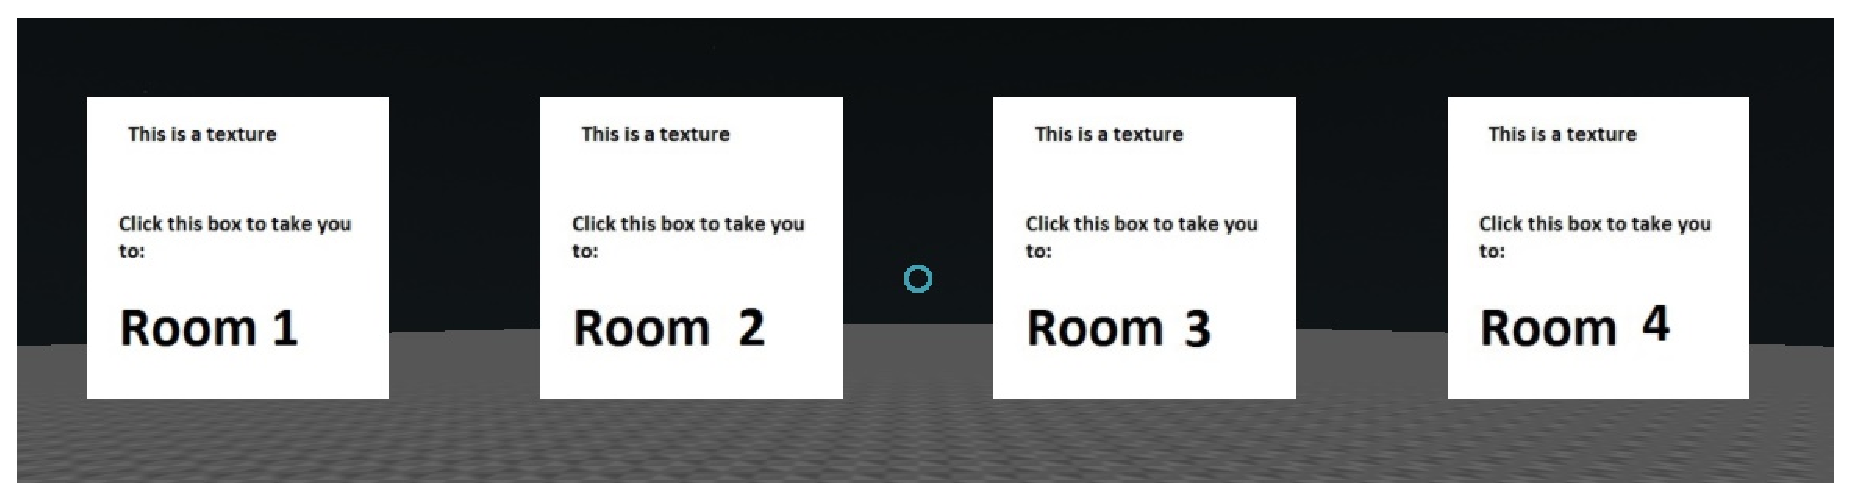
\includegraphics[width=\textwidth]{lobby.eps}\\
\textbf{Figure 1. } The lobby with eight traversal links to new rooms.\\
\vspace{.75cm}
\includegraphics[width=\textwidth]{room1r.eps}\\
\textbf{Figure 2. } Room 1r with multiple trees scattered in the scene.\\
\vspace{.75cm}
\includegraphics[width=\textwidth]{room2r.eps}\\
\textbf{Figure 3. } Room 2r demonstrating some animations (it actually is animated).\\
\vspace{.75cm}
\includegraphics[width=\textwidth]{room3r.eps}\\
\textbf{Figure 4. } Room 3r has some specific user interactions when hovering over the spheres. \\
\vspace{.75cm}
\includegraphics[width=\textwidth]{room4r.eps}\\
\textbf{Figure 4. } Room 4r combines all aspect to put together an interesting scene. \\
\vspace{.75cm}
\end{center}

\end{singlespace}

\end{document}

